
\section{Energy Efficiency}

The STK1000 offers 5 power pin pairs that may be used to measure current consumption of the STK1002 sister board, and therefore also energy efficiency.
These 5 pins are situated on the daughterboard, see figure \ref{power-pins-location}.
Current flow through the pins was measured by connecting an ammeter in series.
Current flow was measured for all five pin pairs on two different versions of the program: the final optimized interrupt-based program, and an earlier busy-wait based program without button cool-down timers.
For both programs current flow was measured twice: once with the program in an idle state, and once where the paddle was moved about by a user frantically pressing \texttt{SW0} and \texttt{SW2} as fast as possible.
The ampere meter used was a BST BS1901W, with a reported accuracy of ±(1.2\% +3d)\cite{BSTBS1901Wmanual}.


The measurements can be found in table \ref{energy-measurements-table}.


\begin{table}
        \begin{tabular}{|l|c|c|c|c|}
                \hline
                              & Interrupt-based &        & Busy-wait-based &        \\
                Pins          & idle            & active & idle            & active \\
                \hline
                \hline
                AVDDUSB (1,2) & 1.77mA          & 1.77mA & 1.77mA          & 1.77mA \\
                \hline
                AVDDPLL (3,4) & 1.97mA          & 1.97mA & 1.97mA          & 1.97mA \\
                \hline
                AVDDOSC (5,6) & 0.00mA          & 0.00mA & 0.00mA          & 0.00mA \\
                \hline
                VDDCORE (7,8) & 30.6mA          & 30.5mA & 26.0mA          & 25.8mA \\
                \hline
                VDDIO (9,10)  & 4.90mA          & 4.99mA & 8.05mA          & 8.13mA \\
                \hline
        \end{tabular}
    \caption{Results of the current consumption measurements of the STK1002}
    \label{energy-measurements-table}
\end{table}

\begin{figure}
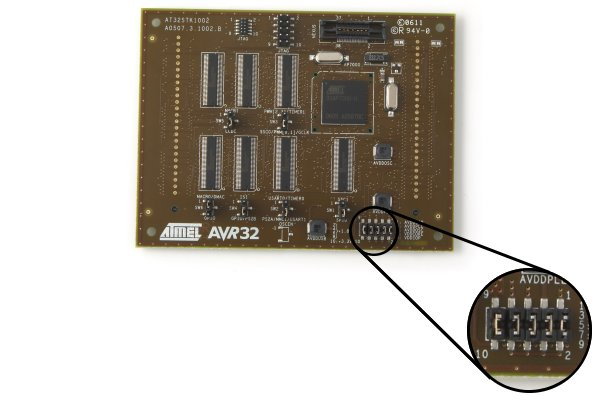
\includegraphics[width = \textwidth]{results-and-tests/power-pins-location.jpg}
\caption{Location of the power pins on the STK1002. Image courtesy of ATMEL.}
\label{power-pins-location}
\end{figure}

VDDCORE (core power supply) and VDDIO (I/O power supply) are the interesting measurements, as AVDDUSB (usb power supply), AVDDPLL (PLL power supply) and AVDDOSC (Oscillator power supply) are not actively affected in the assignment.

Using the sum of the power consumption over VDDCORE and VDDIO during the idle state as an indicator of the total power consumption of the AP7000, we can evaluate the relative energy efficiency performance of the two programs' use of the AP7000.

The power consumption of VDDCORE and VDDIO of the interrupt-based version is 
$
30.6mA \cdot 1.8V +
4.90mA \cdot 3.3V
=
71.3mW
$
.

The power consumption of the busy-wait version is 
$
25.8mA \cdot 1.8V +
8.05mA \cdot 3.3V
=
73mW
$
.


The difference in power consumption is around 2\%, which is near-negligible.

\section{Testing}

	All tests assume that you are in possession of at least one (1) functional STK1000 development board (with cables), a JTAGICE mkII (with USB cable) and a computer with software and hardware capable of interfacing with the JTAGICE.
\paragraph{Button Functionality Test}
This test aims to uncover if pushing Button 0 has the desired effect (the desired effect from pushing Button 0 is that the paddle moves one LED to the right.)
\\ Prerequisites:
\begin{itemize}
	\item One (1) finger
	\item Functional eyesight
\end{itemize}
Procedure:
\begin{enumerate}
	\item Upload the code to the board (e.g using \texttt{make upload}).
	\item Push the board's reset button.
	\item Note the paddle's position.
	\item Push Button 0.
	\item Note the paddle's position.
\end{enumerate}
If the paddle's position in the last step is not one to the right of its position in step \#3, Button 0 does not have the appropriate functionality.
The test can be refactored to test Button 2: simply push Button 2 instead in step \#4 and note that the test will have failed if the paddle's position in step \#5 is not one to the left of its position in step \#3.

\paragraph{Measurement of Power Consumption}
This test measures the board's power consumption by removing a jumper and connecting an amperemeter in series.
The power consumption is to be measured while the board is 
\\
Prerequisites:
\begin{itemize}
	\item{Multimeter or amperemeter}
	\item{Hands, or other tool with similar prehensile ability}
\end{itemize}
Procedure:
\begin{enumerate}
	\item{Turn the STK1000 on and upload your code.}

\section{Discussion}
    
	For the current consumption tests, it is likely that the measuring equipment, as well as methods of measurement, could be improved.
It seems somewhat unlikely that the transition from a busy wait-based approach to an interrupt-based approach should result in only near-negligible differences in power efficiency, based on previous experiences.
One way to measure the current consumption of the entire STK1000 would be to connect a beefier ammeter to the main power supply of the board.
Unfortunately, further investigation of the currency consumption measurements falls outside of the scope of these authors' resources.

On the topic of energy efficiency, the power consumption could probably be reduced further by reducing the CPU's clock speed (\cite{AT32AP7000-prelim}, pg 933-).

The program's code could be further optimized by rewriting it so that it employs less branches. Branching is expensive in terms of clock cycles, and fewer clock cycles equals lower power consumption.

